\documentclass[conference]{IEEEtran}
\IEEEoverridecommandlockouts
\usepackage{tikz}
\usetikzlibrary{shapes.geometric, arrows}
\usepackage{cite}
\usepackage{amsmath,amssymb,amsfonts}
\usepackage{algorithm}
\usepackage{algpseudocode}
\usepackage{graphicx}
\usepackage{textcomp}
\usepackage{xcolor}
\usepackage{pgfplots}
\usepackage{subfigure}

\pgfplotsset{compat=1.9}

\pgfplotsset{
    % #1: index in the group(0,1,2,...)
    % #2: number of plots of that group
    bar group size/.style 2 args={
        /pgf/bar shift={%
                % total width = n*w + (n-1)*skip
                % -> subtract half for centering
                -0.5*(#2*\pgfplotbarwidth + (#2-1)*\pgfkeysvalueof{/pgfplots/bar group skip})  + 
                % the '0.5*w' is for centering
                (.5+#1)*\pgfplotbarwidth + #1*\pgfkeysvalueof{/pgfplots/bar group skip}},%
    },
    bar group skip/.initial=2pt,
    plot 0/.style={cyan,fill=cyan!30!white,mark=none},%
    plot 1/.style={red,fill=red!30!white,mark=none},%
    plot 2/.style={brown!60!black,fill=brown!30!white,mark=none},%
    plot 3/.style={brown!60!black,fill=brown!30!white,mark=none},%
}

\def\BibTeX{{\rm B\kern-.05em{\sc i\kern-.025em b}\kern-.08em
    T\kern-.1667em\lower.7ex\hbox{E}\kern-.125emX}}

\makeatletter
\newcommand\fs@norules{\def\@fs@cfont{\bfseries}\let\@fs@capt\floatc@ruled
    \def\@fs@pre{}%
    \def\@fs@post{}%
    \def\@fs@mid{\kern3pt}%
    \let\@fs@iftopcapt\iftrue}
\makeatother

\tikzstyle{Startstop} = [ellipse,minimum width=2cm, minimum height=1cm, text centered, draw=black, fill=white]
\tikzstyle{io} = [trapezium, trapezium left angle=70, trapezium right angle=110, minimum width=2cm, minimum height=1cm, text centered, draw=black, fill=white]
\tikzstyle{process} = [rectangle, minimum width=1cm, minimum height=1cm, text centered, draw=black, fill=white]
\tikzstyle{decision} = [diamond, minimum width=2cm, minimum height=1cm, text centered, draw=black, fill=white]
\tikzstyle{arrow} = [thick,->,>=stealth]

\newcommand\T{\rule{0pt}{2.6ex}}       % Top strut
\newcommand\B{\rule[-1.2ex]{0pt}{0pt}} % Bottom strut

\begin{document}

%%%%%%%%%%%%%%%%%%%%%%%%%%%%%%%%%%%%%%%%%%%%%%%%%%%%%%%%%%%%%%%%%%%%%%%%%%%%%%%%%%%
%%%%%%%%%%%%%%%%%%%%%%%%%%%%%%%%%%%%%% TITLE %%%%%%%%%%%%%%%%%%%%%%%%%%%%%%%%%%%%%%
%%%%%%%%%%%%%%%%%%%%%%%%%%%%%%%%%%%%%%%%%%%%%%%%%%%%%%%%%%%%%%%%%%%%%%%%%%%%%%%%%%%

\title{Improved Global Routing By Using A Star Algorithm\\}

%%%%%%%%%%%%%%%%%%%%%%%%%%%%%%%%%%%%%%%%%%%%%%%%%%%%%%%%%%%%%%%%%%%%%%%%%%%%%%%%%%%
%%%%%%%%%%%%%%%%%%%%%%%%%%%%%%%%%%%%% AUTHORS %%%%%%%%%%%%%%%%%%%%%%%%%%%%%%%%%%%%%
%%%%%%%%%%%%%%%%%%%%%%%%%%%%%%%%%%%%%%%%%%%%%%%%%%%%%%%%%%%%%%%%%%%%%%%%%%%%%%%%%%%

\author{\IEEEauthorblockN{Abdulrahman Khalid\IEEEauthorrefmark{1}, Hossam Ahmed\IEEEauthorrefmark{2}, Mahmoud Mohamed\IEEEauthorrefmark{3} and Muhanad Atef\IEEEauthorrefmark{4}}
\IEEEauthorblockA{Computer Engineering Dept.,
Faculty of Engineering, Cairo University\\
Cairo, Egypt\\
\IEEEauthorrefmark{1}abdulrahman.elshafei98@gmail.com,
\IEEEauthorrefmark{2}hossamahmed201515@gmail.com,
\IEEEauthorrefmark{3}mmmacmp@gmail.com,
\IEEEauthorrefmark{4}muhanad.atef23@gmail.com}}


\maketitle

%%%%%%%%%%%%%%%%%%%%%%%%%%%%%%%%%%%%%%%%%%%%%%%%%%%%%%%%%%%%%%%%%%%%%%%%%%%%%%%%%%%
%%%%%%%%%%%%%%%%%%%%%%%%%%%%%%%%%%%% ABSTRACT %%%%%%%%%%%%%%%%%%%%%%%%%%%%%%%%%%%%%
%%%%%%%%%%%%%%%%%%%%%%%%%%%%%%%%%%%%%%%%%%%%%%%%%%%%%%%%%%%%%%%%%%%%%%%%%%%%%%%%%%%

\begin{abstract}
    In this paper VLSI routing is improved by improving global routing, this can be done by using A-Star with a heuristic cost function that has parameters which affect the time taken by the router on changing instead of Dijkstra's algorithm in finding path, which will reduce the time taken in this process and achieve the minimum wire length, many comparisons are taken in this paper with different algorithms to find the optimum algorithm to be used to achieve both minimum wire length and minimum time taken. From the comparisons of the paper, we can find that using any algorithm is a trade-off as when the taken time is decreased, the wire length is increased and vice versa, so there is no algorithm which is better from the other algorithms in general but using A-Star algorithm with the heuristic function in finding the path is a good approach to be used in global routing as it decreases the routing time and achieves the minimum wire length.
\end{abstract}

%%%%%%%%%%%%%%%%%%%%%%%%%%%%%%%%%%%%%%%%%%%%%%%%%%%%%%%%%%%%%%%%%%%%%%%%%%%%%%%%%%%
%%%%%%%%%%%%%%%%%%%%%%%%%%%%%%%%%%%% KEY WORDS %%%%%%%%%%%%%%%%%%%%%%%%%%%%%%%%%%%%
%%%%%%%%%%%%%%%%%%%%%%%%%%%%%%%%%%%%%%%%%%%%%%%%%%%%%%%%%%%%%%%%%%%%%%%%%%%%%%%%%%%

\begin{IEEEkeywords}
VLSI Routing, Global Routing, Routing Algorithms, Fast Global Routing, Fast Routing Algorithms, Routing Algoritms Comparisons.
\end{IEEEkeywords} 

%%%%%%%%%%%%%%%%%%%%%%%%%%%%%%%%%%%%%%%%%%%%%%%%%%%%%%%%%%%%%%%%%%%%%%%%%%%%%%%%%%%
%%%%%%%%%%%%%%%%%%%%%%%%%%%%%%%%%% INTRODUCTION %%%%%%%%%%%%%%%%%%%%%%%%%%%%%%%%%%%
%%%%%%%%%%%%%%%%%%%%%%%%%%%%%%%%%%%%%%%%%%%%%%%%%%%%%%%%%%%%%%%%%%%%%%%%%%%%%%%%%%%

\section{Introduction}

Routing is a critical step in the physical design process. Until now the optimum solution for VLSI routing has not been achieved yet, so it is considered a very interesting challenging field. It is exactly done in two steps, global routing, and detailed routing, in global routing, A-technique for 3D global routing is to compress a \textit{3D} grid into a \textit{2D} grid and handle \textit{2D} global routing. The obtained solution is then projected back to \textit{3D} by assignment of layers. as introduced in most of modern designs as in \cite{b1}, \cite{b10}, \cite{b3}, \cite{b4}, \cite{b5}, and \cite{b6}, another less common approach is to route on the \textit{3D} grid directly as in \cite{b9} which applies maze algorithm on the \textit{3D} space, also \cite{b14} uses linear programming to apply routing on the \textit{3D} space, although this approach makes good results, it takes a high runtime and solution space. At first global routing is run which is responsible for making an approximate routing for the whole circuit in order to be used as a guide for detailed routing, then the detailed routing is run to make the exact routing for the system. That means if global or detailed routing is improved the whole routing process is improved, but there are many problems that have to be overcome to make a correct routing process. First of all, the scale has to be taken into consideration, as millions of wires exist in a small chip area which means that many kilometers of wires are placed in a very small area, so total wire length has to be minimized as much as possible, also it is known that as the wire length increases the resistance increases as well which means more delay in the chip. There is another problem as circuits are made in nano-scale which means that its geometric will be complex. Another problem is that the routing algorithm has to be applicable for more than one layer with different costs. The direction of wires also has to be taken into consideration as the direction of wires in every layer can be either vertical or horizontal and no diagonal paths, then to go from source 'S' to target 'T' the path taken should be in (vertical | horizontal) directions that specified by the layer (at each layer wires are placed in one direction only), then there is another problem as when a wire goes from layer to another to continue on the perpendicular direction it has to go through via which has a high resistance. DFM (design for manufacturer) rules also have to be achieved. All of these constraints must be taken into consideration with the global routing to achieve a hundred percent of the circuit connections, which means global routing will take a lot of time to achieve all these constraints, and here is the challenge to achieve all the routing specifications with the minimum time taken. 

\begin{figure} 
\centering  
\subfigure[Before routing] {
    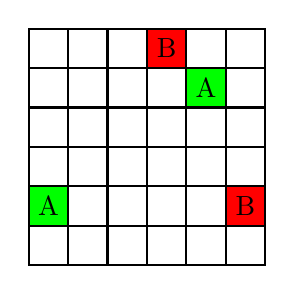
\begin{tikzpicture}
        [
            box/.style={rectangle,draw=black,thick, minimum size=0.5cm},
        ]
    
    \foreach \x in {0,0.5,...,2.5}{
        \foreach \y in {0,0.5,...,2.5}
            \node[box] at (\x,\y){};
    }
    \node [box,fill=green] at (0,0.5){A};
    \node[box,fill=green  ] at (2,2){A};  
    \node[box,fill=red  ] at (1.5,2.5){B}; 
    \node [box,fill=red] at (2.5,0.5){B}; 
    \end{tikzpicture}
}
\subfigure[Iteration number x] {
    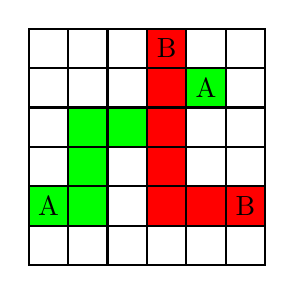
\begin{tikzpicture}
        [
            box/.style={rectangle,draw=black,thick, minimum size=0.5cm},
        ]
    
    \foreach \x in {0,0.5,...,2.5}{
        \foreach \y in {0,0.5,...,2.5}
            \node[box] at (\x,\y){};
    }
    
    \node [box,fill=green] at (0,0.5){A};
    \node[box,fill=green  ] at (2,2){A};  
    \node[box,fill=green  ] at (0.5,0.5){};  
    \node[box,fill=green  ] at (0.5,1){};  
    \node[box,fill=green  ] at (0.5,1.5){};  
    \node[box,fill=green  ] at (1,1.5){};  
    \node[box,fill=red  ] at (1.5,2.5){B}; 
    \node [box,fill=red] at (2.5,0.5){B};
    \node [box,fill=red] at (2,0.5){};
    \node [box,fill=red] at (1.5,0.5){};
    \node [box,fill=red] at (1.5,1){};
    \node [box,fill=red] at (1.5,1.5){};
    \node [box,fill=red] at (1.5,2){};
    \end{tikzpicture}
}
\subfigure[Iteration number y] {
    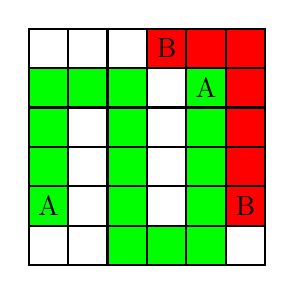
\begin{tikzpicture}
        [
            box/.style={rectangle,draw=black,thick, minimum size=0.5cm},
        ]
    
    \foreach \x in {0,0.5,...,2.5}{
        \foreach \y in {0,0.5,...,2.5}
            \node[box] at (\x,\y){};
    }
    
    \node [box,fill=green] at (0,0.5){A};
    \node[box,fill=green  ] at (2,2){A};  
    \node[box,fill=green  ] at (0,1){};  
    \node[box,fill=green  ] at (0,1.5){};  
    \node[box,fill=green  ] at (0,2){};  
    \node[box,fill=green  ] at (0.5,2){};  
    \node[box,fill=green  ] at (1,2){};  
    \node[box,fill=green  ] at (1,1.5){};  
    \node[box,fill=green  ] at (1,1){};  
    \node[box,fill=green  ] at (1,0.5){};  
    \node[box,fill=green  ] at (1.5,0){};  
    \node[box,fill=green  ] at (1,0){};  
    \node[box,fill=green  ] at (2,0){};  
    \node[box,fill=green  ] at (2,0.5){};  
    \node[box,fill=green  ] at (2,1){};  
    \node[box,fill=green  ] at (2,1.5){};  
    \node[box,fill=red  ] at (1.5,2.5){B}; 
    \node [box,fill=red] at (2.5,0.5){B};  
    \node [box,fill=red] at (2.5,1){};
    \node [box,fill=red] at (2.5,1.5){};
    \node [box,fill=red] at (2.5,2){};
    \node [box,fill=red] at (2.5,2.5){};
    \node [box,fill=red] at (2,2.5){};
    \end{tikzpicture}
}
\subfigure[After N iteration] {
    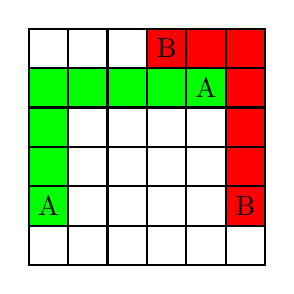
\begin{tikzpicture}
        [
            box/.style={rectangle,draw=black,thick, minimum size=0.5cm},
        ]
    
    \foreach \x in {0,0.5,...,2.5}{
        \foreach \y in {0,0.5,...,2.5}
            \node[box] at (\x,\y){};
    }
    
    \node [box,fill=green] at (0,0.5){A};
    \node[box,fill=green  ] at (2,2){A};  
    \node[box,fill=green  ] at (0,1){};  
    \node[box,fill=green  ] at (0,1.5){};  
    \node[box,fill=green  ] at (0,2){};  
    \node[box,fill=green  ] at (0.5,2){};  
    \node[box,fill=green  ] at (1,2){};  
    \node[box,fill=green  ] at (1.5,2){};  
    \node[box,fill=red  ] at (1.5,2.5){B}; 
    \node [box,fill=red] at (2.5,0.5){B}; 
    \node [box,fill=red] at (2.5,1){};
    \node [box,fill=red] at (2.5,1.5){};
    \node [box,fill=red] at (2.5,2){};
    \node [box,fill=red] at (2.5,2.5){};
    \node [box,fill=red] at (2,2.5){};
    \end{tikzpicture}
}
\caption{Finding path in global routing}
\label{fig:GlobalRoutingProcess}
\end{figure}
\medskip
Figure~\ref{fig:GlobalRoutingProcess} shows a very simple approach of how the global router works. At (a) the source and target of both (A,B) need to be connected ignoring obstacles, nevertheless we can observe that the global router have to iterate to get the best routing paths, at (b) (B,B) connected but there is no way to connect (A,A) as when (B,B) connected together they blocked the way for (A,A) to be connected, after some iterations we can find the figure at (c) in which (A,A) and (B,B) connected correctly, but there is a problem, the (A,A) connection is not the optimal path as there are paths which achieve less wire length, so the global router have to iterate until reaching the optimal path. These iterations are done for only two connections in one layer without obstacles, then how about millions of wires in VLSI? this shows how much the global routing algorithm has to be very fast in order to connect this huge number of wires as fast as possible.


%%%%%%%%%%%%%%%%%%%%%%%%%%%%%%%%%%%%%%%%%%%%%%%%%%%%%%%%%%%%%%%%%%%%%%%%%%%%%%%%%%%
%%%%%%%%%%%%%%%%%%%%%%%%%%%%%%%%%% RELATED WORK %%%%%%%%%%%%%%%%%%%%%%%%%%%%%%%%%%%
%%%%%%%%%%%%%%%%%%%%%%%%%%%%%%%%%%%%%%%%%%%%%%%%%%%%%%%%%%%%%%%%%%%%%%%%%%%%%%%%%%%

\section{Related Work}

Several papers proposed various types of approaches to improve the routing process, each of them tried to improve the overall routing by improving one or more parameters, some papers tried to decrease the number of vias, other papers tried to decrease the time taken and so on.
\medskip
\par
In \cite{b1}, a sequential global routing is used and two bounded length maze algorithms as finding path algorithms are provided in order to make the router faster and to avoid congestions thus avoiding overflow, the first one is optimal-BLMR and the second one is heuristic-BLMR. optimal-BLMR is used to get the minimum cost paths to be used as routing paths, this can be done in three steps. First BLC (bounded length constraint) is defined as a greater number than Manhattan distance then to go from source to target the neighbor points are tested if it can be a part of a path or not, each point that violates the BLC constraint is discarded. Second, if the route Started from point \textit{v}, ended at point \textit{u} and there were many paths between these two points, the normal maze algorithm will take the path with the minimum cost which may cause the route to pass through congestions, but in optimal-BLMR, it keeps track of all paths between these two points in order to choose the path that will not cause overflow, it iterates on the minimum cost path every time and if it found a suitable path it reserves that path, otherwise, it discards that path. Third step the optimal-BLMR iterates on the reserved paths and choose the one to be used for routing. Heuristic-BLMR is used to speed the router up by reserving only one path between the two points, but it has to keep the advantage of optimal-BLMR (avoiding congestions), this can be achieved by reserving the selected path only if the wire length is enough to detour around congested regions. The advantages of this paper are using sequential global routing which is based on multithreaded global routing which speedup the router between $2.71$ and $3.12$ in overflow free cases, avoiding collision by using optimal-BLMR, and making a fast and nearly avoiding collision algorithm (heuristic-BLMR). But there are some disadvantages too, as optimal-BLMR is very slow to be used, although heuristic-BLMR is faster than optimal-BLMR its results are not accurate as the wire length is not the best compared with other papers, and it is done on \textit{2D} grid then it is projected to the \textit{3D} one however, this approach gives a good result but it is not accurate like routers that apply routing in the \textit{3D} grid directly as in \cite{b9}.
\medskip
\par
In \cite{b4}, both of via count and runtime are reduced, this done by integrating \cite{b2}, \cite{b11}, and \cite{b12} with via aware Steiner tree generation, 3-bend routing, and layer assignment with careful edge and net ordering to create \cite{b4}. Via aware Steiner tree is used to at the beginning of the global routing, it generates a suitable topology, by changing tree topology the via count greatly changed, which means that using a suitable topology for Steiner tree will greatly reduce the via count. The 3-bend routing is used instead of L, U, Z, maze, and monotonic routing, as L, U, Z routing can not avoid congestions but they generate a little number of vias, maze and monotonic can avoid congestions but they generate a lot of vias and their runtime is very high, so the 3-bend routing was used as it is fast, its completely \textit{O(nm)}, and it generates vias less than maze and monotonic routing as it consists of two L routing. Layer assignment with careful ordering algorithm is used as a solution of \textit{3D}, it is like all the modern techniques project the \textit{3D} grid into \textit{2D} one to be easier and faster in routing, this algorithm guarantees the wire length and overflow unchanged on assigning to layers, dynamic programming is used in layer assignment to make it faster. From the previous explanation, the advantages of this paper are decreasing the number of vias, which means less power consumption and circuit delay, and decreasing runtime of global routing thus decreasing runtime of whole the routing process. But it has disadvantages too, one of them is the wire length is not optimal, as using 3-bend routing increases the wire length to avoid congestions, another one is caused by layer assignment as if the \textit{2D} was not congestion-free the results will not be accurate.
\medskip
\par
In \cite{b15}, routing efficiency is increased compared to \textit{2D} routers, and runtime is decreased compared to \textit{3D} routers. As the \textit{3D} routers achieve efficient results, it will be used but with some modifications to achieve an acceptable runtime. At first, initialization is done by running a Steiner tree, pattern routing step, and dynamic programming is used in layer assignment as in \textit{2D} routers like \cite{b4}. The second step named coarsening stage, in which, the \textit{3D} grid is split into a hierarchy of levels, a \textit{3D} maze routing is done on each level, starting with the lower level to the higher one, each routed level is projected into the higher one and run the maze algorithm another time to the higher level, which guarantees fewer congestions and less via count as it is a \textit{3D} routing algorithm, 
and the divide and conquer technique they use reduces the time taken. So the advantages of this paper are creating more efficient routing than \textit{2D} and \textit{3D} projection that used in most modern papers and reducing the runtime compared to the ordinary \textit{3D} maze routing. But there are some disadvantages too, one of them that the results are not efficient enough compared to the \textit{3D} routing algorithms, another one is that the runtime still high compared to \textit{2D} routers.  

%%%%%%%%%%%%%%%%%%%%%%%%%%%%%%%%%%%%%%%%%%%%%%%%%%%%%%%%%%%%%%%%%%%%%%%%%%%%%%%%%%%
%%%%%%%%%%%%%%%%%%%%%%%%%%%%%%%% PROPOSED APPROACH %%%%%%%%%%%%%%%%%%%%%%%%%%%%%%%%
%%%%%%%%%%%%%%%%%%%%%%%%%%%%%%%%%%%%%%%%%%%%%%%%%%%%%%%%%%%%%%%%%%%%%%%%%%%%%%%%%%%


\section{Proposed Approach}
For global routing, three parameters are considered. The first is the total wire length, the second is the total overflow. The third is the running time. In our proposed solution, we are focused on the time parameter without affecting much the total wire length and total overflow. So according to minimize the time we have decided to apply A-Star algorithm as the pathfinder algorithm with a proposed heuristic function, A-Star is basically a guided variation of Dijkstra. This algorithm can be turned into a better or worse pathfinding algorithm by experimenting with the heuristics it uses and how it evaluates each node A-Star expands on a node only if it seems promising. Its only focus is to reach the goal node as quickly as possible from the current node, not to try and reach every other node. Illustrative example:
\begin{figure} [hbt!]
    \centering  
    \subfigure[Maze] {
    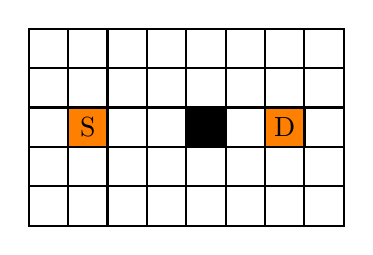
\begin{tikzpicture}
        [
            box/.style={rectangle,draw=black,thick, minimum size=0.5cm},
        ]
    
    \foreach \x in {0,0.5,...,3.5}{
        \foreach \y in {0,0.5,...,2}
            \node[box] at (\x,\y){};
    }
    \node [box,fill=orange] at (0.5,1){S};
    \node[box,fill=orange  ] at (3,1){D};  
    \node[box,fill=black  ] at (2,1){ };  
    \end{tikzpicture}
}

\subfigure[Applying Dijkstra] {
    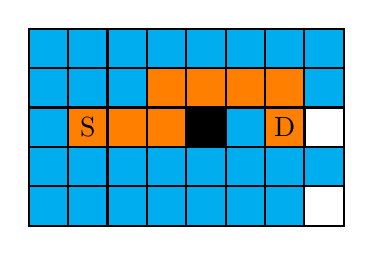
\begin{tikzpicture}
        [
            box/.style={rectangle,draw=black,thick, minimum size=0.5cm},
        ]
    
    \foreach \x in {0,0.5,...,3.5}{
        \foreach \y in {0,0.5,...,2}
            \node[box] at (\x,\y){};
    }

    \node [box,fill=cyan] at (0,0){};
    \node [box,fill=cyan] at (0.5,0){};
    \node [box,fill=cyan] at (1,0){};
    \node [box,fill=cyan] at (1.5,0){};
    \node [box,fill=cyan] at (2,0){};
    \node [box,fill=cyan] at (2.5,0){};
    \node [box,fill=cyan] at (3,0){};
    \node [box,fill=cyan] at (0,0.5){};
    \node [box,fill=cyan] at (0.5,0.5){};
    \node [box,fill=cyan] at (1,0.5){};
    \node [box,fill=cyan] at (1.5,0.5){};
    \node [box,fill=cyan] at (2,0.5){};
    \node [box,fill=cyan] at (2.5,0.5){};
    \node [box,fill=cyan] at (3,0.5){};
    \node [box,fill=cyan] at (3.5,.5){};
    \node [box,fill=cyan] at (2.5,1){};
    \node [box,fill=cyan] at (0,1){};
    \node [box,fill=cyan] at (2.5,0.5){};
    \node [box,fill=cyan] at (0,2){};
    \node [box,fill=cyan] at (0.5,2){};
    \node [box,fill=cyan] at (1,2){};
    \node [box,fill=cyan] at (1.5,2){};
    \node [box,fill=cyan] at (2,2){};
    \node [box,fill=cyan] at (2.5,2){};
    \node [box,fill=cyan] at (3,2){};
    \node [box,fill=cyan] at (3.5,2){};
    \node [box,fill=cyan] at (3.5,1.5){};
    \node [box,fill=cyan] at (0,1.5){};
    \node [box,fill=cyan] at (0.5,1.5){};
    \node [box,fill=cyan] at (1,1.5){};
    \node [box,fill=orange] at (0.5,1){S};
    \node [box,fill=orange] at (1,1){};
    \node [box,fill=orange] at (1.5,1){};
    \node [box,fill=orange] at (1.5,1.5){};
    \node [box,fill=orange] at (2,1.5){};
    \node [box,fill=orange] at (2.5,1.5){};
    \node [box,fill=orange] at (3,1.5){};
    \node[box,fill=orange  ] at (3,1){D};  
    \node[box,fill=black  ] at (2,1){ };  
    \end{tikzpicture}
}
\subfigure[Applying A-Star] {
    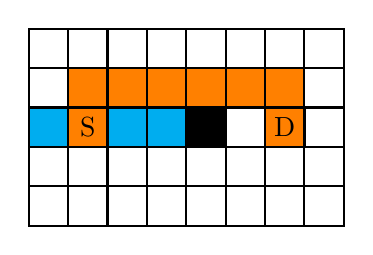
\begin{tikzpicture}
        [
            box/.style={rectangle,draw=black,thick, minimum size=0.5cm},
        ]
    
    \foreach \x in {0,0.5,...,3.5}{
        \foreach \y in {0,0.5,...,2}
            \node[box] at (\x,\y){};
    }
    \node [box,fill=orange] at (0.5,1){S};
    \node[box,fill=orange  ] at (3,1){D};
    \node [box,fill=orange] at (0.5,1.5){};  
    \node [box,fill=orange] at (1,1.5){};  
    \node [box,fill=orange] at (1.5,1.5){};
    \node [box,fill=orange] at (2,1.5){};
    \node [box,fill=orange] at (2.5,1.5){};
    \node [box,fill=orange] at (3,1.5){};
    \node [box,fill=cyan] at (0,1){};
    \node [box,fill=cyan] at (1,1){};
    \node [box,fill=cyan] at (1.5,1){};
    \node[box,fill=black  ] at (2,1){ };  
    \end{tikzpicture}
}
\caption{Comparison between Dijkstra \& A-Star }
\label{fig:GlobalRoutingProcess}
\end{figure}
\medskip
In the illustrative example the visited nodes are marked in cyan color, the path is in orange color, and the blocked cells are black.
Both have path of six cells which in our case they have optimal wire length but totally different running time as Dijkstra visits much more nodes than A-Star
, in the case of many target nodes, Dijkstra might be better in total wire length but much slower than A-Star, with an appropriate heuristic function we can minimize the time and try to reach optimal wire length. The heuristic function is a way of informing the search about the path to a target that provides an intelligent way of guessing which neighbor of the node is going to lead to the target faster. Hence, our heuristic function composed of Manhattan distance, layer index, and some constants.

\begin{multline*}
    h = \ln ((\mid p1 \cdot x-p2 \cdot x\mid+\mid p1 \cdot y-p2 \cdot y\mid)*const1) \\ 
     +(\mid p1 \cdot layerid-p2 \cdot layerid\mid)*const2 \\
\end{multline*}
The global router is implemented using C++ with the boost library, and a parser for LEF/DEF formats. We conducted our experiment with the same configuration and tried to test the global router behavior using A-Star algorithm instead of Dijkstra's.


%%%%%%%%%%%%%%%%%%%%%%%%%%%%%%%%%%%%%%%%%%%%%%%%%%%%%%%%%%%%%%%%%%%%%%%%%%%%%%%%%%%
%%%%%%%%%%%%%%%%%%%%%%%%%%%%%%%%%%%% ALGORITHM %%%%%%%%%%%%%%%%%%%%%%%%%%%%%%%%%%%%
%%%%%%%%%%%%%%%%%%%%%%%%%%%%%%%%%%%%%%%%%%%%%%%%%%%%%%%%%%%%%%%%%%%%%%%%%%%%%%%%%%%

\subsection{Proposed Algorithm}
% \floatstyle{norules}
\restylefloat{algorithm}
\begin{algorithm}[H]
    \caption{A-Star Algorithm}
    \hspace*{\algorithmicindent} \textbf{Input:} Grid values $g$, Source $s$, Destination $d$\\
    \hspace*{\algorithmicindent} \textbf{Output:} Path\\
    \begin{algorithmic}[1]
    \Procedure {A-Star}{}
    % Return  Average waiting time, throughput
    \Statex Declaration and Initialisation:
    \State Cells $\theta$ % The Cells in the grid.
    \State Visited Nodes $\phi$ % Nodes already visited.
    \State Openlist Nodes $\delta$ % Nodes still to be visited. pq
    \State The cost from Starting point to a given node $g$
    \State The heuristic function $h$
    \State (The cost of $g$ + The cost of $h$) is $f$
    \If{$s$ or $d$ is invalid}
        \Return
    \EndIf
    \If{$s$ or $d$ is blocked}
        \Return
    \EndIf
    \If{$s$ = $d$}
        \Return
    \EndIf
    \State Initialize $\delta$ 
    \State Initialize $\phi$
        \While{$\delta$ is not empty}
            \State $currNode$  = node with least $f$ in $\delta$
            \State $\delta$.Remove($currNode$)
            \State Generate 4 neighbours of $currNode$
            \For{$neighbour \in neighbours$}
            \If{$neighbour$ = $d$}
                \State Get path
                \Return
            \ElsIf{$neighbour \notin \phi$ and $neighbour$ is not blocked}
                \State $gnew$ = $currNode$.$g$ + distance between neighbour and currNode
                \State $hnew$ = distance from $d$ to $neighbour$
                \State $fnew$ = $gnew$ + $hnew$
                \If{$fnew < neighbour$.$f$}
                \State $neighbour$.$g$ = $currNode$.$g$ + distance between neighbour and currNode
                \State $neighbour$.$h$ = distance from $d$ to $neighbour$
                \State $neighbour$.$f$ = $neighbour$.$g$ + $neighbour$.$h$
                \State $\delta$.Add($neighbour$)
                \EndIf
            \EndIf
            \EndFor
        \State $\phi$.Add($currNode$)
        \EndWhile
        \EndProcedure
    \end{algorithmic}
\end{algorithm}


%%%%%%%%%%%%%%%%%%%%%%%%%%%%%%%%%%%%%%%%%%%%%%%%%%%%%%%%%%%%%%%%%%%%%%%%%%%%%%%%%%%
%%%%%%%%%%%%%%%%%%%%%%%%%%%%%% EXPERIMENTAL ANALYSIS %%%%%%%%%%%%%%%%%%%%%%%%%%%%%%
%%%%%%%%%%%%%%%%%%%%%%%%%%%%%%%%%%%%%%%%%%%%%%%%%%%%%%%%%%%%%%%%%%%%%%%%%%%%%%%%%%%

\section{Experimental Analysis}

%%%%%%%%%%%%%%%%%%%%%%%%%%%%%%%%%%%%%%%%%%%%%%%%%%%%%%%%%%%%%%%%%%%%%%%%%%%%%%%%%%%
%%%%%%%%%%%%%%%%%%%%%%%%%%%%%%%%%%% ASSUMPTIONS %%%%%%%%%%%%%%%%%%%%%%%%%%%%%%%%%%%
%%%%%%%%%%%%%%%%%%%%%%%%%%%%%%%%%%%%%%%%%%%%%%%%%%%%%%%%%%%%%%%%%%%%%%%%%%%%%%%%%%%

\subsection{Assumptions}

The proposed scheduling algorithm is software simulated using a Python script which simulates scheduling independent CPU-bound processes on a single processor environment which guarantees that no more than a single process is getting scheduled at any arbitrary moment. Each process is assumed to have its own predetermined burst time, arrival time and the queue to which each one belongs. The proposed approach is non-preemptive. For the sake of giving an example, if a process was lately introduced to a queue denoted by $Q_{i}$ prior to the current queue getting scheduled, it won't get scheduled until the current queue, its subsequent queues and the queues prior to $Q_{i}$ get scheduled.

%%%%%%%%%%%%%%%%%%%%%%%%%%%%%%%%%%%%%%%%%%%%%%%%%%%%%%%%%%%%%%%%%%%%%%%%%%%%%%%%%%%
%%%%%%%%%%%%%%%%%%%%%%%%%%%%%%%%%%%%%%% I/O %%%%%%%%%%%%%%%%%%%%%%%%%%%%%%%%%%%%%%%
%%%%%%%%%%%%%%%%%%%%%%%%%%%%%%%%%%%%%%%%%%%%%%%%%%%%%%%%%%%%%%%%%%%%%%%%%%%%%%%%%%%

\subsection{Experimental Scheme}

On one hand, the input arguments to the proposed algorithm implementation are the number of processes to be scheduled, their burst time, their arrival time and the queue where each one belongs. On the other hand, output parameters are the average waiting time, average turnaround time and throughput. The following equations are used to calculate the previously mentioned output parameters:

\begin{equation}
    Average\; Waiting\; Time =  \frac{Total \; Waiting \; Time}{Number \; of \; Processes} \label{eq2}
\end{equation}

\begin{equation}
    Average\; Turnaround\; Time =  \frac{Total \; Turnaround \; Time}{Number \; of \; Processes} \label{eq3}
\end{equation}

\begin{equation}
    Throughput =  \frac{Number \; of \; Executed \; Processes}{Total \; Execution \; Time} \label{eq4}
\end{equation}

% \vspace{4mm}

%%%%%%%%%%%%%%%%%%%%%%%%%%%%%%%%%%%%%%%%%%%%%%%%%%%%%%%%%%%%%%%%%%%%%%%%%%%%%%%%%%%
%%%%%%%%%%%%%%%%%%%%%%%%%%%%%%% PERFORMANCE METRICS %%%%%%%%%%%%%%%%%%%%%%%%%%%%%%%
%%%%%%%%%%%%%%%%%%%%%%%%%%%%%%%%%%%%%%%%%%%%%%%%%%%%%%%%%%%%%%%%%%%%%%%%%%%%%%%%%%%

\subsection{Performance Metrics}

As a means to have a concrete, viable evaluation of either the proposed algorithm or any other scheduling algorithm, the output parameters are taken into consideration for analysis. Since the average waiting time indicates the average time that a  process had to Starve for, therefore the lower the average waiting time is the better. The same principle applies to the average turnaround time and the number of context switches, as the former implies the average time spent by the process since its arrival time to its completion and the latter costs time as the CPU is assigned back and forth between different processes. Contrarily to the prior metrics, the larger the throughput is the better as it indicates the number of processes that are completely executed per unit time.

%%%%%%%%%%%%%%%%%%%%%%%%%%%%%%%%%%%%%%%%%%%%%%%%%%%%%%%%%%%%%%%%%%%%%%%%%%%%%%%%%%%
%%%%%%%%%%%%%%%%%%%%%%%%%%%%%%%%%%% SIMULATION %%%%%%%%%%%%%%%%%%%%%%%%%%%%%%%%%%%%
%%%%%%%%%%%%%%%%%%%%%%%%%%%%%%%%%%%%%%%%%%%%%%%%%%%%%%%%%%%%%%%%%%%%%%%%%%%%%%%%%%%

\subsection{Simulation}

For the sake of showcasing the proposed algorithm, a number of processes, their predetermined burst time values and their arrival time values are taken as input to the Python simulation script. Suppose that the input to the script is according to the following table:

\begin{table}[H]
    \caption{}
    \centering
     \begin{tabular}{||c c c c||} 
     \hline
     \textit{\textbf{Process}} & \textit{\textbf{Arrival Time}} & \textit{\textbf{Burst Time}} & \textit{\textbf{Queue}} \T \B \\ 
     \hline
     \hline
     1 & 0 & 60 & 1 \T \B \\ 
     \hline
     2 & 0 & 50 & 1 \T \B \\
     \hline
     3 & 0 & 40 & 2 \T \B \\
     \hline
     4 & 0 & 30 & 2 \T \B \\
     \hline
     5 & 0 & 10 & 3 \T \B \\ 
     \hline
     6 & 0 & 210 & 3 \T \B \\ 
     \hline
     7 & 0 & 200 & 3 \T \B \\ 
     \hline
     \end{tabular}
     \label{table1}
\end{table}

According to the proposed algorithm, the time quanta calculated are as follows:

\begin{table}[H]
    \caption{}
    \centering
     \begin{tabular}{||c c||} 
     \hline
     \textit{\textbf{Queue}} & \textit{\textbf{Quantum Value}} \T \B \\ 
     \hline
     \hline
     1 & 55 \T \B \\ 
     \hline
     2 & 40 \T \B \\
     \hline
     3 & 615 \T \B \\
     \hline
     4 & 0 \T \B \\
     \hline
     5 & 0 \T \B \\ 
     \hline
     \end{tabular}
\end{table}

All processes are sorted in ascending order according to their remaining time and are scheduled by assigning the time quantum calculated for their respective queue. The time spent scheduling a particular queue is the waiting time for its subsequent queues.

The scheduling process goes as follows:

\begin{figure}[H]
        \begin{center}
        \begin{tabular}{|c|c|}
         \hline
            $P_{2}$ & $P_{1}$\T\B\\ 
         \hline
        \end{tabular}
        \end{center}
        \begin{center}
            \begin{tabular}{c c c}
                   0 & 50 & 105\\ 
            \end{tabular}
        \end{center}
    \caption{$Q_{1}$ Gantt Chart}
\end{figure}

Considering that each process in $Q_{1}$ is assigned a quantum value of $50$, as we reach the last process in $Q_{1}$, the total time elapsed equals $105$, which happens to be the time that all the other processes in the subsequent queues had to wait for, hence the addition of their waiting time by a value of $105$ units of time.

\begin{figure}[H]
    \begin{center}
    \begin{tabular}{|c|c|c|c|}
     \hline
        $P_{1}$ & $P_{5}$ & $P_{4}$ & $P_{3}$\T\B\\ 
     \hline
    \end{tabular}
    \end{center}
    \begin{center}
        \begin{tabular}{c c c c c}
               105 & 110 & 120 & 150 & 190\\ 
        \end{tabular}
    \end{center}
\caption{$Q_{2}$ Gantt Chart}
\end{figure}



\begin{figure}[H]
    \begin{center}
    \begin{tabular}{|c|c|}
     \hline
        P7 & P6\T\B\\ 
     \hline
    \end{tabular}
    \end{center}
    \begin{center}
        \begin{tabular}{c c c}
               190 & 390 & 600\\ 
        \end{tabular}
    \end{center}
\caption{$Q_{3}$ Gantt Chart}
\end{figure}

Whenever processes reach the lowest queue precompletion, they are scheduled using the RR scheduling algorithm with a relatively large quantum time value which is in most cases similar to using the FCFS algorithm because, as the time quantum value of an RR algorithm tends to infinity which could practically be a very large number relative to the available processes remaining time values, the algorithm tends to morph into the FCFS algorithm. This procedure is iterated until all the processes are finished. Simulation results are shown in the table below:

\begin{table}[H]
    \caption{}
    \centering
     \begin{tabular}{||c c c||} 
     \hline
     \textit{\textbf{Avg. Turnaround Time}} & \textit{\textbf{Avg. Waiting Time}} & \textit{\textbf{Throughput}}\T \B \\ 
     \hline
     \hline
     230 & 144.3 & 0.011667 \T \B \\ 
     \hline
     \end{tabular}
\end{table}

%%%%%%%%%%%%%%%%%%%%%%%%%%%%%%%%%%%%%%%%%%%%%%%%%%%%%%%%%%%%%%%%%%%%%%%%%%%%%%%%%%%
%%%%%%%%%%%%%%%%%%%%%%%%%%%%%%%%%%% COMPARISONS %%%%%%%%%%%%%%%%%%%%%%%%%%%%%%%%%%%
%%%%%%%%%%%%%%%%%%%%%%%%%%%%%%%%%%%%%%%%%%%%%%%%%%%%%%%%%%%%%%%%%%%%%%%%%%%%%%%%%%%

\subsection{Performance Comparisons}

To assess the performance of the proposed algorithm implementation, multiple test cases are addressed and analyzed in seven different experiments. In each experiment, the output of the proposed algorithm implementation is compared to the output of another scheduling algorithm implementation addressed in a different paper, such as standard MLFQ algorithm with static quantum RR and other variants of MLFQ algorithms and RR algorithms.

\subsubsection{Experiment 1}

In this experiment, the proposed algorithm is compared against two MLFQ algorithm variants stated in {b4}. The first uses a static version of the RR algorithm for scheduling each queue, while the second variant uses a dynamic version of the RR algorithm for doing so.

\begin{table}[H]
    \caption{Experiment 1 Input}
    \centering
     \begin{tabular}{||c c c c||} 
     \hline
     \textit{\textbf{Process}} & \textit{\textbf{Arrival Time}} & \textit{\textbf{Burst Time}} & \textit{\textbf{Queue}} \T \B \\ 
     \hline
     \hline
     1 & 1 & 25 & 1 \T \B \\ 
     \hline
     2 & 5 & 70 & 1 \T \B \\
     \hline
     3 & 6 & 84 & 1 \T \B \\
     \hline
     4 & 7 & 17 & 1 \T \B \\
     \hline
     5 & 8 & 35 & 1 \T \B \\ 
     \hline
     \end{tabular}
\end{table}

\begin{table}[H]
    \caption{Experiment 1 Results}
    \centering
    \begin{tabular}{||c c c||}
        \hline
        \textit{\textbf{Algorithm}} & \textit{\textbf{Avg. Turnaround Time}} & \textit{\textbf{Avg. Waiting Time}}\T \B \\
    \hline
    \hline
    \textbf{Proposed Algorithm} & 115 & 68.8 \T \B\\ \hline
    \textbf{Dynamic RR MLFQ} & 150.8 & 107.6\T \B\\ \hline
    \textbf{Static RR MLFQ} & 161.4 & 116.2 \T \B\\ \hline
     \end{tabular}
\end{table}

\subsubsection{Experiment 2}

In this experiment, the proposed algorithm is compared against two MLFQ algorithm variants stated in {b4}. The first uses a static version of the SJFRR algorithm for scheduling each queue, while the second variant uses a dynamic version of the SJFRR algorithm for doing so. 

\begin{table}[H]
    \caption{Experiment 2 Input}
    \centering
     \begin{tabular}{||c c c c||} 
     \hline
     \textit{\textbf{Process}} & \textit{\textbf{Arrival Time}} & \textit{\textbf{Burst Time}} & \textit{\textbf{Queue}} \T \B \\ 
     \hline
     \hline
     1 & 1 & 25 & 1 \T \B \\ 
     \hline
     2 & 5 & 70 & 1 \T \B \\
     \hline
     3 & 6 & 84 & 1 \T \B \\
     \hline
     4 & 7 & 17 & 1 \T \B \\
     \hline
     5 & 8 & 35 & 1 \T \B \\ 
     \hline
     \end{tabular}
\end{table}

\begin{table}[H]
    \caption{Experiment 2 Results}
    \centering
    \begin{tabular}{||c c c||}
        \hline
        \textit{\textbf{Algorithm}} & \textit{\textbf{Avg. Turnaround Time}} & \textit{\textbf{Avg. Waiting Time}}\T \B \\
    \hline
    \hline
    \textbf{Proposed Algorithm} & 115 & 68.8 \T \B\\ \hline
    \textbf{Dyn. SJFRR MLFQ} & 134 & 91.8\T \B\\ \hline
    \textbf{Stat. SJFRRMLFQ} & 143.4 & 98.2 \T \B\\ \hline
     \end{tabular}
\end{table}

\subsubsection{Experiment 3}

In this experiment, the proposed algorithm is compared against two MLFQ algorithm variants stated in {b5}. The first uses a static version of the SJFRR algorithm for scheduling each queue, while the second variant uses a dynamic version of the SJFRR algorithm for doing so.

\begin{table}[H]
    \caption{Experiment 3 Input}
    \centering
     \begin{tabular}{||c c c c||} 
     \hline
     \textit{\textbf{Process}} & \textit{\textbf{Arrival Time}} & \textit{\textbf{Burst Time}} & \textit{\textbf{Queue}} \T \B \\ 
     \hline
     \hline
     1 & 0 & 8 & 1 \T \B \\ 
     \hline
     2 & 3 & 133 & 3 \T \B \\
     \hline
     3 & 2 & 21 & 2 \T \B \\
     \hline
     4 & 8 & 39 & 2 \T \B \\
     \hline
     5 & 19 & 67 & 2 \T \B \\ 
     \hline
     6 & 33 & 114 & 3 \T \B \\ 
     \hline
     7 & 33 & 54 & 2 \T \B \\ 
     \hline
     \end{tabular}
\end{table}

\begin{table}[H]
    \caption{Experiment 3 Results}
    \centering
    \begin{tabular}{||c c c||}
        \hline
        \textit{\textbf{Algorithm}} & \textit{\textbf{Avg. Turnaround Time}} & \textit{\textbf{Avg. Waiting Time}}\T \B \\
    \hline
    \hline
    \textbf{Proposed Algorithm} & 151 & 88.7 \T \B\\ \hline
    \textbf{Dyn. SJFRR MLFQ} & 252 & 119 \T \B\\ \hline
    \textbf{Stat. SJFRR MLFQ} & 351 & 228 \T \B\\ \hline
     \end{tabular}
\end{table}

\subsubsection{Experiment 4}

In this experiment, the proposed algorithm is compared against multiple variants of the MLFQ algorithm that are stated in {b6}: standard MLFQ algorithm, a priority-based MLFQ algorithm and a vague logic-based MLFQ algorithm.

\begin{table}[H]
    \caption{Experiment 4 Input}
    \centering
     \begin{tabular}{||c c c c||} 
     \hline
     \textit{\textbf{Process}} & \textit{\textbf{Arrival Time}} & \textit{\textbf{Burst Time}} & \textit{\textbf{Queue}} \T \B \\ 
     \hline
     \hline
     1 & 0 & 40 & 1 \T \B \\ 
     \hline
     2 & 0 & 30 & 1 \T \B \\
     \hline
     3 & 0 & 50 & 1 \T \B \\
     \hline
     4 & 2 & 70 & 1 \T \B \\
     \hline
     5 & 4 & 25 & 1 \T \B \\ 
     \hline
     6 & 6 & 60 & 1 \T \B \\ 
     \hline
     7 & 7 & 45 & 1 \T \B \\ 
     \hline
     \end{tabular}
\end{table}

\begin{table}[H]
    \caption{Experiment 4 Results} 
    \centering
    \begin{tabular}{||c c c||}
        \hline
        \textit{\textbf{Algorithm}} & \textit{\textbf{Avg. Turnaround Time}} & \textit{\textbf{Avg. Waiting Time}}\T \B \\
    \hline
    \hline
    \textbf{Proposed Algorithm} & 185.85 & 140.14 \T \B\\ \hline
    \textbf{VMLFQ} & 190 & 170 \T \B\\ \hline
    \textbf{MLFQ} & 232.14 & 175 \T \B\\ \hline
    \textbf{PMLFQ} & 240 & 180 \T \B\\ \hline
     \end{tabular}
\end{table}

\subsubsection{Experiment 5}

This experiment is the same as the previous one, but with a different input test case. 

\begin{table}[H]
    \caption{Experiment 5 Input}
    \centering
     \begin{tabular}{||c c c c||} 
     \hline
     \textit{\textbf{Process}} & \textit{\textbf{Arrival Time}} & \textit{\textbf{Burst Time}} & \textit{\textbf{Queue}} \T \B \\ 
     \hline
     \hline
     1 & 0 & 90 & 1 \T \B \\ 
     \hline
     2 & 0 & 30 & 1 \T \B \\
     \hline
     3 & 0 & 28 & 1 \T \B \\
     \hline
     4 & 0 & 57 & 1 \T \B \\
     \hline
     5 & 0 & 73 & 1 \T \B \\ 
     \hline
     6 & 0 & 19 & 1 \T \B \\ 
     \hline
     7 & 0 & 42 & 1 \T \B \\ 
     \hline
     8 & 0 & 67 & 1 \T \B \\ 
     \hline
     \end{tabular}
\end{table}

\begin{table}[H]
    \caption{Experiment 5 Results}
    \centering
    \begin{tabular}{||c c c||}
        \hline
        \textit{\textbf{Algorithm}} & \textit{\textbf{Avg. Turnaround Time}} & \textit{\textbf{Avg. Waiting Time}}\T \B \\
    \hline
    \hline
    \textbf{Proposed Algorithm} & 212.5 & 161.75 \T \B\\ \hline
    \textbf{VMLFQ} & 260 & 225 \T \B\\ \hline
    \textbf{MLFQ} & 290 & 240 \T \B\\ \hline
    \textbf{PMLFQ} & 300 & 245 \T \B\\ \hline
     \end{tabular}
\end{table}

\subsubsection{Experiment 6}

In this experiment, the proposed algorithm is compared against two variants of the RR algorithm stated in {b3}. The first is a static version of the RR algorithm with a constant quantum value of $25$ for scheduling each queue while the second uses a dynamic version of the RR algorithm called SRBRR for doing so. 

\begin{table}[H]
    \caption{Experiment 6 Input}
    \centering
     \begin{tabular}{||c c c c||} 
     \hline
     \textit{\textbf{Process}} & \textit{\textbf{Arrival Time}} & \textit{\textbf{Burst Time}} & \textit{\textbf{Queue}} \T \B \\ 
     \hline
     \hline
     1 & 0 & 13 & 1 \T \B \\ 
     \hline
     2 & 0 & 35 & 1 \T \B \\
     \hline
     3 & 0 & 46 & 1 \T \B \\
     \hline
     4 & 0 & 63 & 1 \T \B \\
     \hline
     5 & 0 & 97 & 1 \T \B \\ 
     \hline
     \end{tabular}
\end{table}

\begin{table}[H]
    \caption{Experiment 6 Results}
    \centering
    \begin{tabular}{||c c c||}
        \hline
        \textit{\textbf{Algorithm}} & \textit{\textbf{Avg. Turnaround Time}} & \textit{\textbf{Avg. Waiting Time}}\T \B \\
    \hline
    \hline
    \textbf{Proposed Algorithm} & 113.2 & 62.4 \T \B\\ \hline
    \textbf{Dynamic SRBRR} & 122.4 & 71.6 \T \B\\ \hline
    \textbf{Static RR} & 148.2 & 97.4 \T \B\\ \hline
     \end{tabular}
\end{table}

\subsubsection{Experiment 7}

This experiment is the same as the previous one, but with a different input test case. Note that for this test case, a process queue number is irrelevant to both the RR algorithm and the SRBRR algorithm mentioned in {b3}.

\begin{table}[H]
    \caption{Experiment 7 Input}
    \centering
     \begin{tabular}{||c c c c||} 
     \hline
     \textit{\textbf{Process}} & \textit{\textbf{Arrival Time}} & \textit{\textbf{Burst Time}} & \textit{\textbf{Queue}} \T \B \\ 
     \hline
     \hline
     1 & 0 & 54 & 1 \T \B \\ 
     \hline
     2 & 0 & 99 & 3 \T \B \\
     \hline
     3 & 0 & 5 & 2 \T \B \\
     \hline
     4 & 0 & 27 & 2 \T \B \\
     \hline
     5 & 0 & 32 & 2 \T \B \\ 
     \hline
     \end{tabular}
\end{table}

\begin{table}[H]
    \caption{Experiment 7 Results}
    \centering
    \begin{tabular}{||c c c||}
        \hline
        \textit{\textbf{Algorithm}} & \textit{\textbf{Avg. Turnaround Time}} & \textit{\textbf{Avg. Waiting Time}}\T \B \\
    \hline
    \hline
    \textbf{Dynamic SRBRR} & 93.6 & 50.2 \T \B\\ \hline
    \textbf{Proposed Algorithm} & 106.8 & 63.4 \T \B\\ \hline
    \textbf{Static RR} & 152.2 & 108.8 \T \B\\ \hline
     \end{tabular}
\end{table}

%%%%%%%%%%%%%%%%%%%%%%%%%%%%%%%%%%%%%%%%%%%%%%%%%%%%%%%%%%%%%%%%%%%%%%%%%%%%%%%%%%%
%%%%%%%%%%%%%%%%%%%%%%%%%%%%%%%%%%% OBSERVATION %%%%%%%%%%%%%%%%%%%%%%%%%%%%%%%%%%%
%%%%%%%%%%%%%%%%%%%%%%%%%%%%%%%%%%%%%%%%%%%%%%%%%%%%%%%%%%%%%%%%%%%%%%%%%%%%%%%%%%%

\subsection{Observation}

From the above simulations of different test cases and multiple performance comparisons that involved as many as 11 different scheduling algorithms not including this paper algorithm, it is clear that the average turnaround time and the average waiting time of the proposed algorithm is less than or – in few occasions  – nearly equal to those of the stated algorithms. With that said, the proposed algorithm is arguably advantageous over those algorithms, considering even the case in which it underperformed compared to the SRBRR algorithm, it is still favourable due to the capability to separate processes into categories based on their need for the processor and other advantages of the MLFQ algorithm. The performance of the proposed algorithm compared to other algorithms is further illustrated in the following graphs:

\begin{figure}[H]
    \begin{center}
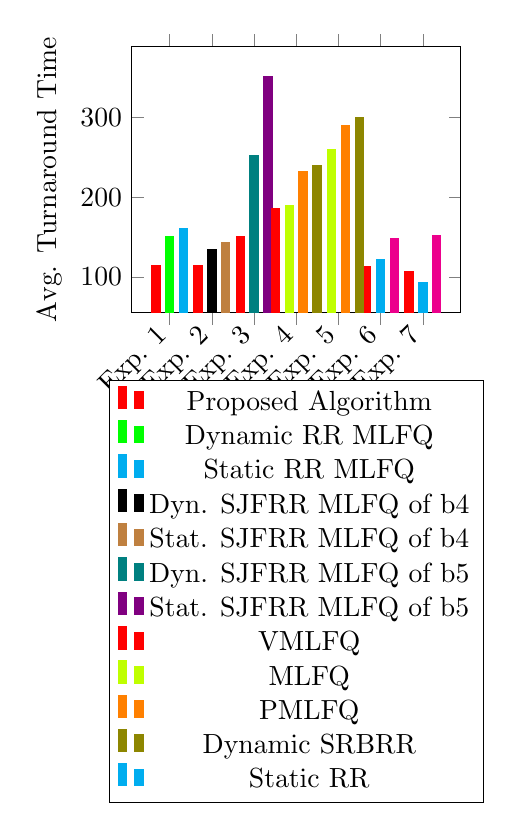
\begin{tikzpicture}
    \begin{axis}[
        width=0.475*\textwidth,
        symbolic x coords={Exp. 1,Exp. 2,Exp. 3,Exp. 4,Exp. 5,Exp. 6,Exp. 7},
        ylabel=Avg. Turnaround Time,
        enlargelimits=0.15,
        legend style={at={(0.5,-0.25)}, anchor=north,legend columns=1},
        ybar,
        xtick={Exp. 1,Exp. 2,Exp. 3,Exp. 4,Exp. 5,Exp. 6,Exp. 7},
        x tick label style={rotate=45,anchor=east},
        bar width=3pt,
        cycle list name=color list
    ]

    \addplot[plot 0,bar group size={0}{3}, red]
    coordinates {(Exp. 1,115) (Exp. 2,115) (Exp. 3,151) (Exp. 6,113.2) (Exp. 7,106.8)};
    \addplot[plot 1,bar group size={1}{3}, green]
    coordinates {(Exp. 1,150.8)};
    \addplot[plot 2,bar group size={2}{3}, cyan]
    coordinates {(Exp. 1,161.4)};

    \addplot[plot 1,bar group size={1}{3}, black]
    coordinates {(Exp. 2,134)};
    \addplot[plot 2,bar group size={2}{3}, brown]
    coordinates {(Exp. 2,143.4)};

    \addplot[plot 1,bar group size={1}{3}, teal]
    coordinates {(Exp. 3,252)};
    \addplot[plot 2,bar group size={2}{3}, violet]
    coordinates {(Exp. 3,351)};

    \addplot[plot 0,bar group size={0}{4}, red]
    coordinates {(Exp. 4,185.85) (Exp. 5,212.5)};
    \addplot[plot 1,bar group size={1}{4}, lime]
    coordinates {(Exp. 4,190) (Exp. 5,260)};
    \addplot[plot 2,bar group size={2}{4}, orange]
    coordinates {(Exp. 4,232.14) (Exp. 5,290)};
    \addplot[plot 3,bar group size={3}{4}, olive]
    coordinates {(Exp. 4,240) (Exp. 5,300)};

    \addplot[plot 1,bar group size={1}{3}, cyan]
    coordinates {(Exp. 6,122.4) (Exp. 7,93.6)};
    \addplot[plot 2,bar group size={2}{3}, magenta]
    coordinates {(Exp. 6,148.2) (Exp. 7,152.2)};
    
    \legend{Proposed Algorithm,Dynamic RR MLFQ, Static RR MLFQ, Dyn. SJFRR MLFQ of {b4},  Stat. SJFRR MLFQ of {b4}, Dyn. SJFRR MLFQ of {b5}, Stat. SJFRR MLFQ of {b5}, VMLFQ, MLFQ, PMLFQ, Dynamic SRBRR, Static RR}
    \end{axis}
\end{tikzpicture}
\end{center}
\caption{Comparison graph for average turnaround time}
\vspace{45mm}
\end{figure}

\begin{figure}[H]
    \begin{center}
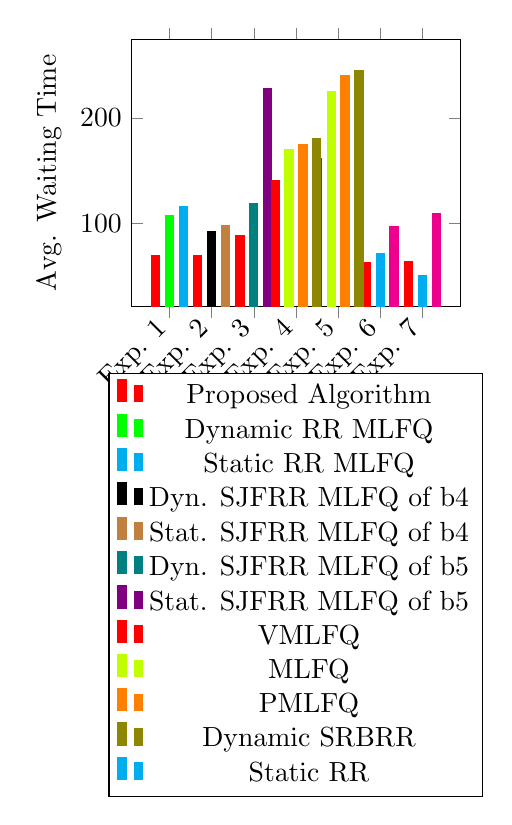
\begin{tikzpicture}
    \begin{axis}[
        width=0.475*\textwidth,
        symbolic x coords={Exp. 1,Exp. 2,Exp. 3,Exp. 4,Exp. 5,Exp. 6,Exp. 7},
        ylabel=Avg. Waiting Time,
        enlargelimits=0.15,
        legend style={at={(0.5,-0.25)}, anchor=north,legend columns=1},
        ybar,
        xtick={Exp. 1,Exp. 2,Exp. 3,Exp. 4,Exp. 5,Exp. 6,Exp. 7},
        x tick label style={rotate=45,anchor=east},
        bar width=3pt,
        cycle list name=color list
    ]

    \addplot[plot 0,bar group size={0}{3}, red]
    coordinates {(Exp. 1,68.8) (Exp. 2,68.8) (Exp. 3,88.7) (Exp. 6,62.4) (Exp. 7,63.4)};
    \addplot[plot 1,bar group size={1}{3}, green]
    coordinates {(Exp. 1,107.6)};
    \addplot[plot 2,bar group size={2}{3}, cyan]
    coordinates {(Exp. 1,116.2)};

    \addplot[plot 1,bar group size={1}{3}, black]
    coordinates {(Exp. 2,91.8)};
    \addplot[plot 2,bar group size={2}{3}, brown]
    coordinates {(Exp. 2,98.2)};

    \addplot[plot 1,bar group size={1}{3}, teal]
    coordinates {(Exp. 3,119)};
    \addplot[plot 2,bar group size={2}{3}, violet]
    coordinates {(Exp. 3,228)};

    \addplot[plot 0,bar group size={0}{4}, red]
    coordinates {(Exp. 4,140.14) (Exp. 5,161.75)};
    \addplot[plot 1,bar group size={1}{4}, lime]
    coordinates {(Exp. 4,170) (Exp. 5,225)};
    \addplot[plot 2,bar group size={2}{4}, orange]
    coordinates {(Exp. 4,175) (Exp. 5,240)};
    \addplot[plot 3,bar group size={3}{4}, olive]
    coordinates {(Exp. 4,180) (Exp. 5,245)};

    \addplot[plot 1,bar group size={1}{3}, cyan]
    coordinates {(Exp. 6,71.6) (Exp. 7,50.2)};
    \addplot[plot 2,bar group size={2}{3}, magenta]
    coordinates {(Exp. 6,97.2) (Exp. 7,108.8)};
    
    \legend{Proposed Algorithm,Dynamic RR MLFQ, Static RR MLFQ, Dyn. SJFRR MLFQ of {b4},  Stat. SJFRR MLFQ of {b4}, Dyn. SJFRR MLFQ of {b5}, Stat. SJFRR MLFQ of {b5}, VMLFQ, MLFQ, PMLFQ, Dynamic SRBRR, Static RR}
    \end{axis}
\end{tikzpicture}
\end{center}
\caption{Comparison graph for average waiting time}
\end{figure}

%%%%%%%%%%%%%%%%%%%%%%%%%%%%%%%%%%%%%%%%%%%%%%%%%%%%%%%%%%%%%%%%%%%%%%%%%%%%%%%%%%%
%%%%%%%%%%%%%%%%%%%%%%%%%%%%%%%%%%% CONCLUSION %%%%%%%%%%%%%%%%%%%%%%%%%%%%%%%%%%%%
%%%%%%%%%%%%%%%%%%%%%%%%%%%%%%%%%%%%%%%%%%%%%%%%%%%%%%%%%%%%%%%%%%%%%%%%%%%%%%%%%%%

\section{Conclusion and Future Work}

In the process of physical design, routing is among the most critical steps and is usually a very challenging problem. Effective and powerful routing algorithms are important to deal with the challenges emerging from the increasingly growing scale of IC integration, Routers will continue to evolve with rapidly growing design challenges like signal integrity, nanometer effects, reliability, etc. The goal of this paper is to develop A-Star-based global Router with minimum wire length and the number of vias as the more vias number the more heat generated from the chip with minimum run time. In order to optimize the time parameter, we use a heuristic function that decreases the run time of router and test it with different constants to define its effect on run time, for future work we aim to define an effective heuristic function to improve the running time. And build upon A-Star algorithm using more efficient versions of A-Star algorithm such as bi-directional A-Star, iterative deepening A-Star. In bi-directional A-Star that processes edges in both directions that improve the running time as well as it saves the memory demand for path saving as we will deal with both directions of edge.

%%%%%%%%%%%%%%%%%%%%%%%%%%%%%%%%%%%%%%%%%%%%%%%%%%%%%%%%%%%%%%%%%%%%%%%%%%%%%%%%%%%
%%%%%%%%%%%%%%%%%%%%%%%%%%%%%%%%%%%% REFERENCES %%%%%%%%%%%%%%%%%%%%%%%%%%%%%%%%%%%
%%%%%%%%%%%%%%%%%%%%%%%%%%%%%%%%%%%%%%%%%%%%%%%%%%%%%%%%%%%%%%%%%%%%%%%%%%%%%%%%%%%

\begin{thebibliography}{00}

    \bibitem{b1} Liu, Wen-Hao, et al. "NCTU-GR 2.0: Multithreaded collision-aware global routing with bounded-length maze routing." \textit{IEEE Transactions on computer-aided design of integrated circuits and systems} 32.5 (2013): 709-722.
    
    \bibitem{b2} Zhang, Yanheng, Yue Xu, and Chris Chu. "FastRoute3. 0: a fast and high quality global router based on virtual capacity." \textit{2008 IEEE/ACM International Conference on Computer-Aided Design.} IEEE, 2008.

    \bibitem{b3} H.-Y. Chen, C.-H. Hsu, and Y.-W. Chang, “High-performance global routing with fast overflow reduction,” \textit{in 2009 Asia and South Pacific Design Automation Conference}, pp. 582–587, IEEE, 2009.

    \bibitem{b4} Xu, Yue, Yanheng Zhang, and Chris Chu. "FastRoute 4.0: global router with efficient via minimization." \textit{2009 Asia and South Pacific Design Automation Conference. IEEE}, 2009.

    \bibitem{b5} Cho, Minsik, et al. "BoxRouter 2.0: Architecture and implementation of a hybrid and robust global router." \textit{2007 IEEE/ACM International Conference on Computer-Aided Design. IEEE}, 2007.

    \bibitem{b6} Ozdal, Muhammet Mustafa, and Martin DF Wong. "Archer: a history-driven global routing algorithm." \textit{2007 IEEE/ACM International Conference on Computer-Aided Design. IEEE}, 2007.

    \bibitem{b7} Gao, Jhih-Rong, Pei-Ci Wu, and Ting-Chi Wang. "A new global router for modern designs." \textit{2008 Asia and South Pacific Design Automation Conference.} IEEE, 2008.

    \bibitem{b8} Moffitt, Michael D. "MaizeRouter: Engineering an effective global router." \textit{IEEE Transactions on Computer-Aided Design of Integrated Circuits and Systems} 27.11 (2008): 2017-2026.

    \bibitem{b9} Roy, Jarrod A., and Igor L. Markov. "High-performance routing at the nanometer scale." \textit{IEEE Transactions on Computer-Aided Design of Integrated Circuits and Systems} 27.6 (2008): 1066-1077.

    \bibitem{b10} Chang, Yen-Jung, Yu-Ting Lee, and Ting-Chi Wang. "NTHU-Route 2.0: a fast and stable global router." \textit{2008 IEEE/ACM International Conference on Computer-Aided Design. IEEE}, 2008.

    \bibitem{b11} Pan, Min, and Chris Chu. "FastRoute: A step to integrate global routing into placement." \textit{Proceedings of the 2006 IEEE/ACM international conference on Computer-aided design.} 2006.

    \bibitem{b12} Pan, Min, and Chris Chu. "FastRoute 2.0: A high-quality and efficient global router." \textit{2007 Asia and south pacific design automation conference.} IEEE, 2007.

    \bibitem{b13} Liu, Jinwei, et al. "CUGR: Detailed-Routability-Driven 3D Global Routing with Probabilistic Resource Model."

    \bibitem{b14} Wu, Tai-Hsuan, Azadeh Davoodi, and Jeffrey T. Linderoth. "GRIP: scalable 3D global routing using integer programming." \textit{Proceedings of the 46th Annual Design Automation Conference}. 2009.

    \bibitem{b15} Xu, Yue, and Chris Chu. "MGR: Multi-level global router." \textit{2011 IEEE/ACM International Conference on Computer-Aided Design (ICCAD)}. IEEE, 2011.

\end{thebibliography}

\end{document}
